\SSbreak\\
\emph{Source: 2007 Sharygin Correspondence Round 18}\\
\emph{Proposer: \Paiya}\\ %\Pchan \Pbrain \Pss
\emph{Problem ID: 195}\\
\emph{Date: 2021-05-23}\\
\emph{Difficulty: Challenging}\\
\SSbreak
 
\SSpsetQ{
    $O, G$ are points in the plane such that $OG = 20.21$. Let $S$ be the set of vertices of all triangles with positive area that have circumcentre $O$ and centre of mass $G$,
and $T$ the set of points in the plane that are not in $S$. If the area of $T$ is $U$, find $\lfloor 100U \rfloor$.
    \begin{center}
        \textit{(A scientific calculator may be used.)}
    \end{center}
    %Put Problem Here
}\bigskip

\begin{solution}\hfil\medskip
	
    The \href{https://geometry.ru/olimp/2007/zaochsol.pdf}{official solution} is in Russian. I don't understand Russian. \medskip

    The main motivation here is the Euler Line and the points on it. 

    \textit{Euler Line.} $O, G, H$, circumcentre, centre of mass, and orthocentre of a triangle, are collinear with $2OG = GH$ or all three coincident. 
    Consider the homothety that sends each vertex of $\triangle ABC$ to the midpoint of its opposite side, thus sending $\triangle ABC$ to its 
    medial triangle; this homothety is then centered at $G$ (why?). Then, $H$ is mapped to the orthocentre of the medial triangle, but this point is
    the circumcentre of $\triangle ABC$. \medskip

    \textit{Lemma.} Let $F$ be the midpoint of $\overline{AB}$. Then, $CH = 2OF$. This is closely related with the proof of the existence of the nine-point-circle.
    Consider the homothety centered at $N_9$ that sends $O$ to $H$; this homothety has scale $-1$. Then, $F$ is sent to the midpoint of $\overline{CH}$ since the foot
    of the $C$-altitude is on the nine-point-circle, implying that $F$ and the midpoint of $\overline{CH}$ are diametrically opposite. We are done. \medskip

    But note that $OF < R$, so we have the constraint $CH = 2OF < 2R = 2OC$. The locus for which $\frac{CH}{OC} \leq 2$ is a union of Apollonian circles forming 
    a disk with the boundary circle being the Apollonian circle where $\frac{CH}{OC} = 2$. Two diametrically opposite points on this circle are $G$ and $G'$, where
    $G'$ is on the Euler line and $G'O = 60.63$, making the disk have radius $40.42$. To construct such $\triangle ABC$, let $F$ be the point on $\overrightarrow{CG}$ such that
    $CF > CG$ and $CG = 2GF.$ Then draw a line at $F$ perpendicular to $\overline{OF}$ and a circle centered at $O$ with radius $OC$; the points $A, B$ are the 
    intersections of circle and line. \medskip

    \begin{center}
        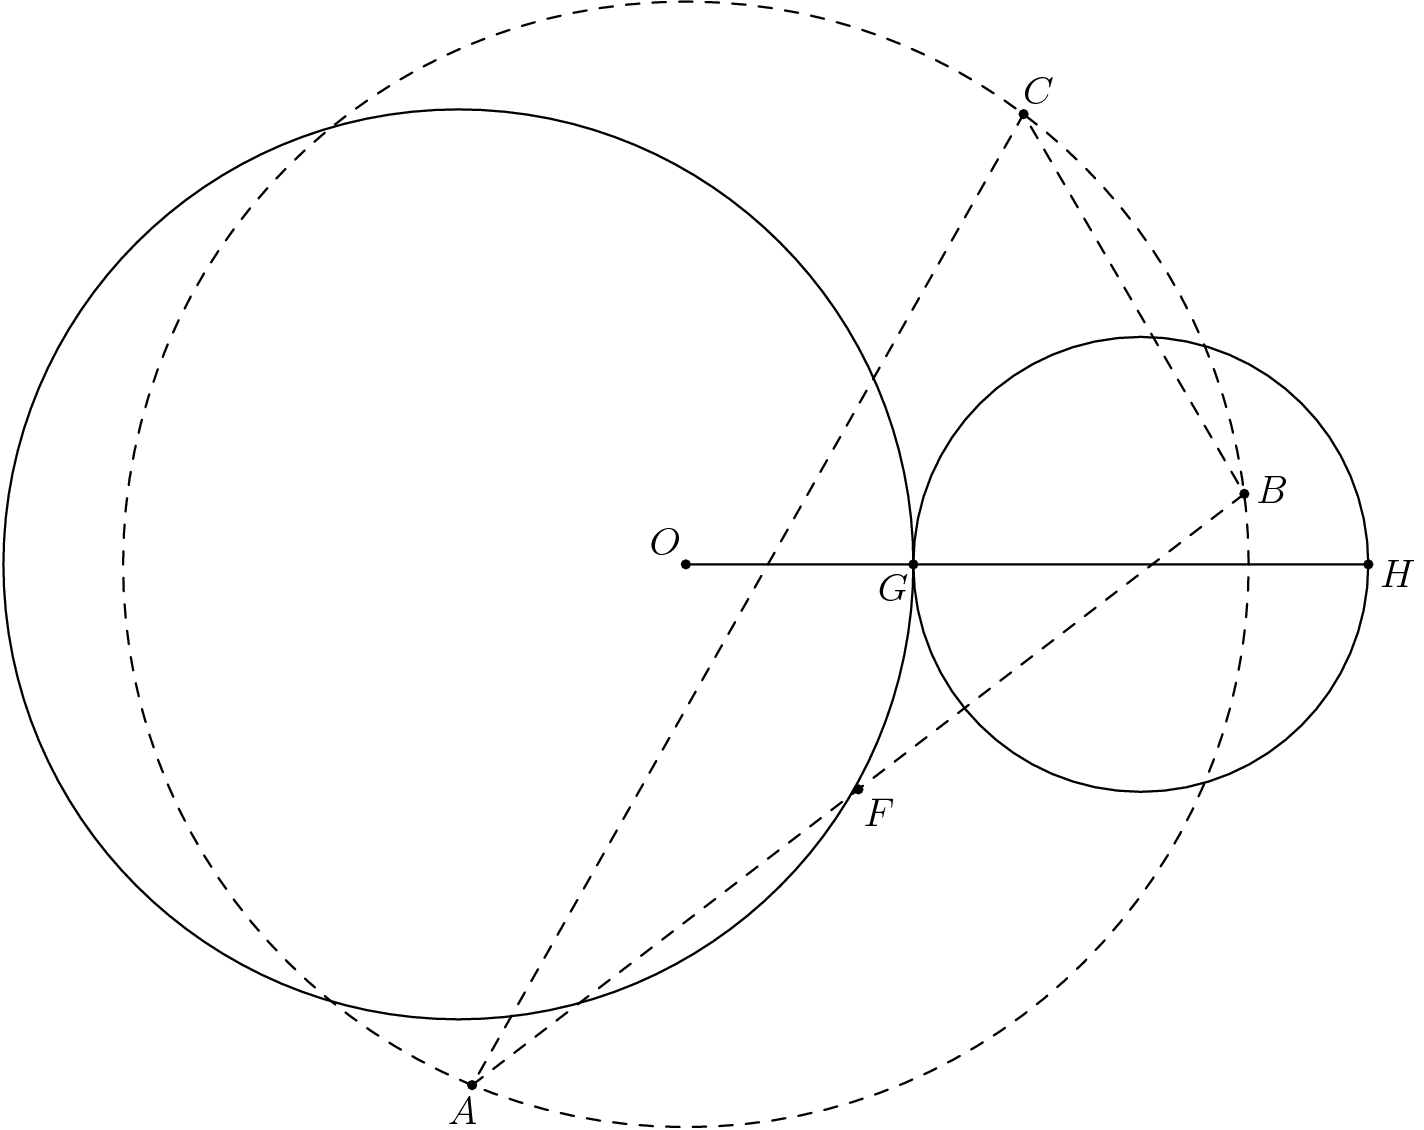
\includegraphics[scale=0.4]{Sections/Files/14-1-7.png}
    \end{center}

    We are missing one detail: what if $A, B, C$ are all collinear? Then, since $\overline{FO} \parallel \overline{CH}$ we have $\angle CFO = \angle GCH$, 
    but since $A, B, C$ collinear we have $\angle CFO = 90$, or, $C$ is on the circle with diameter $\overline{GH}$, which in our case has radius $20.21$
    and does not intersect the aforementioned disk. \medskip
    
    Our answer is $100\pi\left(40.42^2 + 20.21^2\right) \iff \boxed{641582}.$ \medskip

    \textit{Remark.} RDS-1 was the first Soviet nuke. 
    %Put sol here
\end{solution}\bigskip
